\newpage
\pagenumbering{arabic}
\setcounter{page}{4}
\section{Introduction}

\subsection{Focus area}
This rapport is a project in the subject "ELE-510 Image Processing with Robot Vision". The original task were "Detection of one known object", like a dog. However this rapport will focus on recognition of objects using an convolutional neural networks (CNN). This means that recognition of any form of object the neural network is trained to detect, will be tried to be detected. This mean optimally it will not only recognise one single object, but those object it is designed to recognise. 

\subsection{Object detection and recognition}
Since the focus area of this rapport will be object recognition and not object detection, it is important to know the difference between those two terms. 

\subsubsection*{Object detection}
Object detection, is detecting one certain object given it is in the picture. For a program designed to detect number plates, the input should be an image containing a number plate. Then the output should be a bounding box around the number plate, if it exist. Or it could be the position of the number plate to be used later. One use for this type could be an automated toll station who need the number plate of the vehicles driving trough the toll station.

This mean that object detection only can detect what it is supposed to detect.

\begin{figure}%
    \centering
        \subfloat[Object detection]{{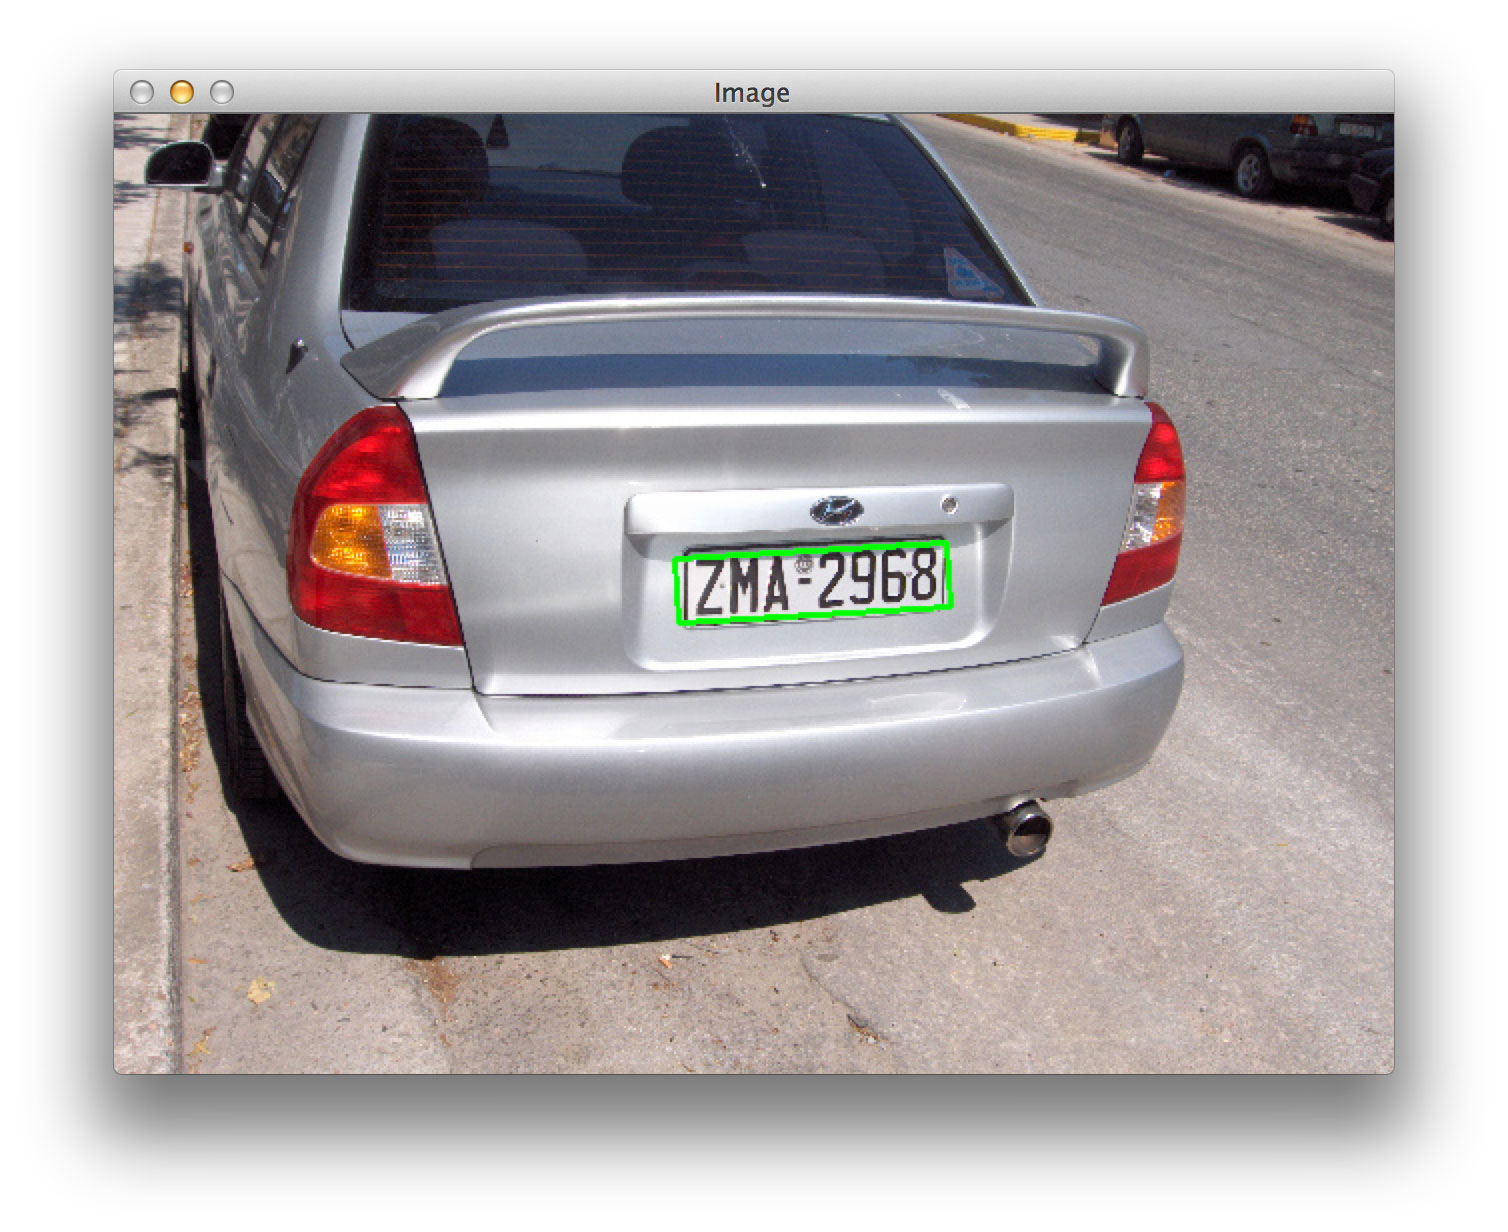
\includegraphics[width=6.5cm]{img/license_detection.jpg} }}
    \qquad
        \subfloat[Object recognition]{{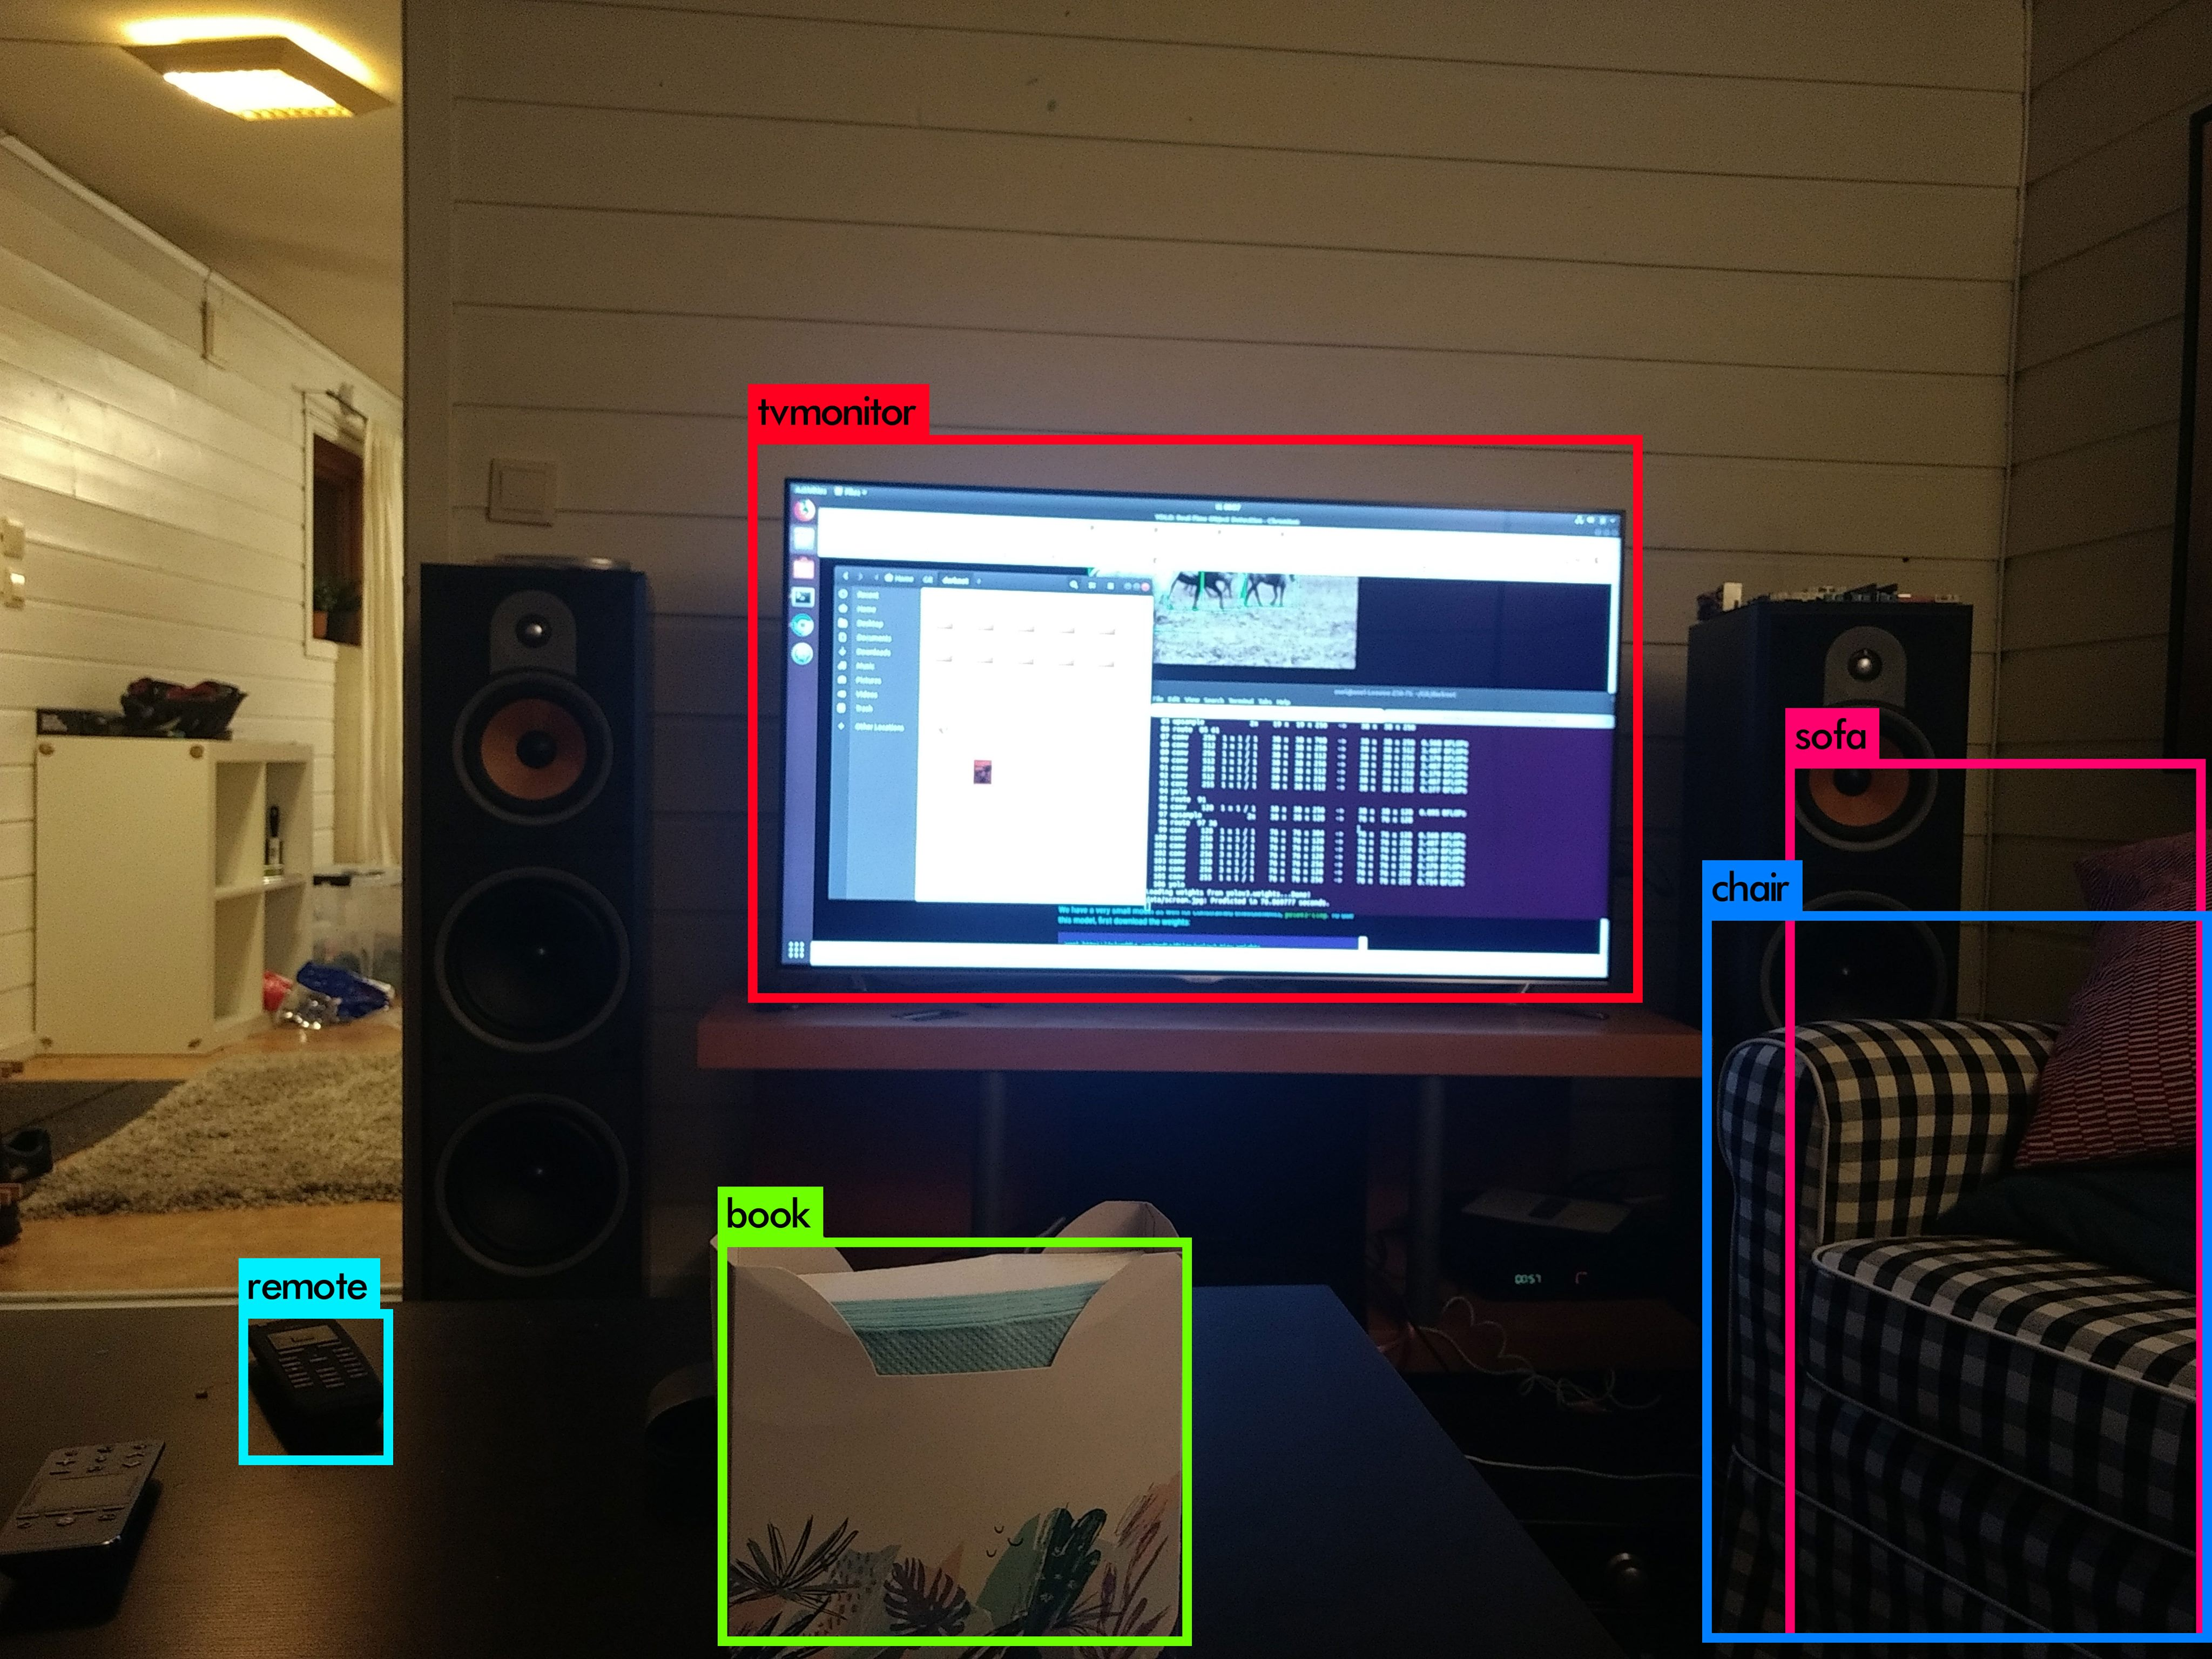
\includegraphics[width=6.5cm]{img/or.jpg} }}
    \caption{Object detection and object recognition}
    \label{fig:OdVsOr}
\end{figure}

\subsubsection*{Object recognition}
Object recognition is recognising different objects in an image or video. A typical input is a video stream or an image, and the output will be bounding boxes around images with a marker telling what the object is. Like for instance, car, bird, person. This mean that object recognition can detect and distinguish what kind of object there is in the sample.

Now there is multiple ways using object recognition, but the widely used methods is by "Machine Learning" or by "Convolutional Neural Networks".

\subsection{ Why YOLO algorithm}
This rapport will focus on the "You Only Look Once" algorithm [referanse] by now only called YOLO. YOLO is a quite fast and accurate object recognition algorithm utilising CNN to detect objects. This is as fast as 30-120 images per seconds on a nvidia Titan X GPU. The variation of fps is due to the use of different weights in neural networks. In easier terms this means the accuracy can be reduced in change with higher refresh rate. \textit{The high refresh rate of the YOLO make this quite interesting and popular. }